\documentclass{article}
\usepackage[utf8]{inputenc}
\usepackage[brazil]{babel}
\usepackage{graphicx}
\usepackage{amsmath, amssymb}
\usepackage{hyperref}
\usepackage{float}
\usepackage[a4paper, margin=1in]{geometry} 
\usepackage{setspace}
\onehalfspacing


\title{Fundamentos de Probabilidade e Estatística para Ciência de Dados}
\author{Resumo das aulas do Prof. Dr. Francisco Rodrigues (ICMC-USP)}
\date{Agosto de 2025}

\begin{document}

% Capa personalizada
\begin{titlepage}
    \centering
    \vspace*{3cm}
    {\scshape\LARGE Universidade de São Paulo \par}
    \vspace{1cm}
    {\scshape\Large Instituto de Ciências Matemáticas e de Computação\par}
    \vspace{2.5cm}
    {\huge\bfseries Fundamentos de Probabilidade e Estatística para Ciência de Dados\par}
    \vspace{1cm}
    {\Large Resumo das aulas do Prof. Dr. Francisco Rodrigues\par}
    \vfill
    {\Large Bruna Zamith Santos\par}
    \vspace{0.5cm}
    {\large Agosto de 2025\par}
\end{titlepage}

% Sumário
\tableofcontents
\newpage

\section{Teoria dos Conjuntos}
Sejam os conjuntos:
\[
A = \{1, 2, 4, 9\}, \quad B = \{3, 7, 9\}
\]

\begin{itemize}
  \item União: $A \cup B = \{1, 2, 3, 4, 7, 9\}$
  \item Interseção: $A \cap B = \{7, 9\}$
  \item Complementar de $B$: $B^C = \{1, 2, 4\}$
  \item Complementar de $A$: $A^C = \{3, 7\}$
  \item Espaço amostral ($\Omega$): É o conjunto de todos os resultados possíveis de um experimento aleatório. Exemplo: $\Omega = \{1, 2, 3, 4, 5, 6\}$, ao lançar um dado.
  \item Evento ($A$): É um subconjunto do espaço amostral. Exemplo: $A = \{2, 4, 6\}$
  \item Evento impossível ($\emptyset$): É um evento que nunca ocorre.
  \item Evento certo ($\Omega$): É o evento que sempre ocorre.
  \item $A \cup B$: É o evento que ocorre se $A$ ou $B$ (ou ambos) ocorrerem.
  \item $A \cap B$: É o evento que ocorre se $A$ e $B$ ocorrerem ao mesmo tempo.
  \item $A^C$: É o evento que ocorre se $A$ não ocorre.
  \item Eventos mutuamente exclusivos: Quando $A \cap B = \emptyset$.
\end{itemize}

\section{Experimento Aleatório}
Um experimento aleatório é um experimento que pode ser repetido inúmeras vezes sob as mesmas condições, sendo o seu resultado incerto.

\section{Conceitos de Probabilidade}
Sejam $\Omega$ o espaço amostral e $A$ um evento em $\Omega$. Então, uma função $P(\cdot)$ é denominada probabilidade se satisfaz:
\begin{itemize}
    \item $0 \leq P(A) \leq 1$, $\forall A \in \Omega$ 
    \item $P(\Omega) = 1$
    \item Se $A_1, A_2, \dots$ forem eventos mutuamente exclusivos, isto é, $A_i \cap A_j = \emptyset$, $\forall i \neq j$, então:
    $$
    P\left( \bigcup_{i=1}^{\infty} A_i \right) = \sum_{i=1}^{\infty} P(A_i)
    $$
\end{itemize}

Se um experimento aleatório tiver $n(\Omega)$ resultados mutuamente exclusivos e igualmente possíveis, e se um evento $A$ conter $n(A)$ desses resultados, a probabilidade de ocorrência desse evento é definida por:
    $$
    P(A) = \frac{n(A)}{n(\Omega)} = \frac{|A|}{|\Omega|}
    $$

Sejam $A$ e $B$ eventos em um mesmo espaço amostral, então:

\begin{itemize}
  \item $P(\emptyset) = 0$
  \item $P(A) = 1 - P(A^C)$
  \item Se $A \subseteq B$, então $P(A) \leq P(B)$
\end{itemize}

\subsection{Probabilidade Frequentista}
A probabilidade de um evento é igual à sua frequência de ocorrência em um grande número de experimentos:
    $$
    P(A) = \lim_{n \to \infty} \frac{n_A}{n}
    $$,
onde $n_A$ é o número de vezes que o evento $A$ ocorre em $n$ experimentos.

\subsection{Probabilidade de União de Dois Eventos}
Para dois eventos $A$ e $B$ em um mesmo espaço amostral:
    $$
    P(A \cup B) = P(A) + P(B) - P(A \cap B)
    $$

\subsection{Probabilidade Condicional}

Sejam dois eventos $A$ e $B$ em um mesmo espaço amostral $\Omega$.  
A probabilidade condicional de $A$ dado que $B$ ocorreu é definida por:
    $$
    P(A \mid B) = \frac{P(A \cap B)}{P(B)}, \quad \text{com } P(B) > 0
    $$

Assim, $A$ e $B$ são eventos independentes se, e somente se:
    $$
    P(A \cap B) = P(A) \cdot P(B)
    $$

Ou equivalentemente:
    $$
    P(A \mid B) = P(A) \quad \text{e} \quad P(B \mid A) = P(B)
    $$

\subsection{Partições do Espaço Amostral}
Os eventos $B_1, B_2, \dots, B_n$ formam uma partição do espaço amostral $\Omega$ se:

\begin{itemize}
    \item $B_i \cap B_j = \emptyset$, para $i \neq j$, com $i, j = 1, \dots, n$
    \item $\bigcup_{i=1}^n B_i = \Omega$
    \item $P(B_i) \geq 0$, para $i = 1, \dots, n$
\end{itemize}

Seja $A$ um evento no espaço amostral $\Omega$ e seja $B_1, \dots, B_n$ uma partição amostral de $\Omega$. Podemos escrever $A$ considerando tal partição:
    $$
    A = \bigcup_{i=1}^n (A \cap B_i)
    $$
    $$
    P(A) = P\left( \bigcup_{i=1}^n A \cap B_i \right) = \sum_{i=1}^n P(A \cap B_i)
    $$

Sejam $B_1, B_2, \dots, B_n$ uma partição do espaço amostral $\Omega$. Então, qualquer evento $A \subseteq \Omega$ pode ser escrito como:
    $$
    P(A) = \sum_{i=1}^n P(A \mid B_i) \cdot P(B_i)
    $$

\section{Teorema de Bayes}
Sejam $B_1, B_2, \dots, B_n$ uma partição do espaço amostral $\Omega$, e $A$ um evento com $P(A) > 0$, então:
    $$
    P(B_i \mid A) = \frac{P(A \mid B_i) \cdot P(B_i)}{\sum_{j=1}^n P(A \mid B_j) \cdot P(B_j)}
    $$

E assim podemos definir:
    $$
    P(A \mid B) = \frac{P(B \mid A) \cdot P(A)}{P(B)}
    $$

\section{Variáveis Aleatórias}
Suponha que lancemos dois dados. O espaço amostral associado ao experimento, sendo os eventos $C$: ``sai uma cara'' e $R$: ``sai uma coroa'', é dado por:

$$
\Omega = \{CC, CR, RC, RR\}
$$

Uma possível variável aleatória associada ao experimento é definida por:
$$
X = \text{``número de caras obtido no experimento''}
$$

\begin{itemize}
    \item Representamos variáveis aleatórias por letras maiúsculas ($X, Y, Z$), enquanto usamos letras minúsculas para indicar os valores das variáveis ($x, y, z$).
    \item Se o número de valores possíveis de uma variável aleatória for finito ou infinito enumerável, dizemos que é uma variável aleatória discreta.
    \item Caso contrário, é uma variável aleatória contínua.
\end{itemize}

A função que atribui a cada valor da variável aleatória sua respectiva probabilidade é chamada de distribuição de probabilidade:
    $$
    P(X = x_i) = p(x_i) = p_i, \quad i = 1,2,3
    $$

A distribuição de probabilidade também é chamada de função massa de probabilidade. E temos que:
    $$
    \sum_{i=1}^{n} P(X = x_i) = 1
    $$

Dizemos que $X$ é uma variável aleatória contínua se existir uma função $f$ denominada função densidade de probabilidade (fdp) que satisfaz:
\begin{itemize}
    \item $f(x) \geq 0, \quad \forall x \in \mathbb{R}$
    \item $\int_{-\infty}^{\infty} f(x) \, dx = 1$
    \item $P(a \leq X \leq b) = \int_{a}^{b} f(x) \, dx
    $, $-\infty < a < b < \infty$
    \item $f(x)$ é uma função com valores positivos e área unitária.
\end{itemize}

Seja $X$ uma variável aleatória discreta ou contínua. A probabilidade condicional de que $X \in S$ dado que $X \in V$ é:
    $$
    P(X \in S \mid X \in V) = \frac{P(X \in S \cap V)}{P(X \in V)}
    $$,
onde $S$ e $V$ são subconjuntos do espaço da variável.

\section{Função de Distribuição}
A função distribuição acumulada ou simplesmente função de distribuição de uma variável aleatória $X$ é definida por:
    $$
    F(x) = P(X \leq x)
    $$

Se discreta:
    $$
    F(x) = \sum_{x_i \leq x} P(X = x_i)
    $$

Se contínua:
    $$
    F(x) = \int_{-\infty}^{x} f(t) \, dt
    $$

Propriedades da função de distribuição:
\begin{itemize}
    \item $0 \leq F(x) \leq 1, \quad F(x) \text{ é não decrescente}$,
    \item $\lim_{x \to -\infty} F(x) = 0, \quad \lim_{x \to +\infty} F(x) = 1$
    \item Caso discreto: $P(a < X \leq b) = F(b) - F(a)$
    \item Caso contínuo: $f(x) = \frac{dF(x)}{dx}$
\end{itemize}

\section{Esperança}
\subsection{Variável Aleatória Discreta}
Seja $X$ uma variável aleatória discreta com distribuição de probabilidade $P(X = x_i)$. O valor esperado (ou esperança matemática) é:
    $$
    E[X] = \sum_{i=1}^{n} x_i \cdot P(X = x_i)
    $$

\subsection{Variável Aleatória Contínua}
Seja $X$ uma variável aleatória contínua com função densidade de probabilidade $f(x)$, então:
    $$
    E[X] = \int_{-\infty}^{+\infty} x \cdot f(x) \, dx
    $$

\subsection{Função de uma Variável Aleatória}
Seja $g(X)$ uma função de uma variável aleatória discreta $X$. Então:
    $$
    E[g(X)] = \sum_{i=1}^{n} g(x_i) \cdot P(X = x_i)
    $$

Seja $g(X)$ uma função de variável contínua com densidade $f(x)$. Então:
    $$
    E[g(X)] = \int_{-\infty}^{\infty} g(x) \cdot f(x) \, dx
    $$

\subsection{Propriedades}
\begin{itemize}
    \item Se $X = c$, onde $c$ é constante, então: $E[X] = E[c] = c$
    \item Se $c$ é constante: $E[cX] = c \cdot E[X]$
    \item Então: $E[aX + b] = a \cdot E[X] + b$
\end{itemize}

\section{Momento}
\subsection{Momento Estatístico}
Seja $X$ uma variável aleatória discreta com valores $x_1, x_2, \dots, x_k$. O momento de ordem $n$ de $X$ é:
    $$
    E[X^n] = \sum_{i=1}^{k} x_i^n \cdot P(X = x_i)
    $$

Se $X$ for contínua:
    $$
    E[X^n] = \int_{-\infty}^{\infty} x^n f(x) \, dx
    $$

\subsection{Momento Central}
Seja $X$ uma variável aleatória.

\begin{itemize}
    \item Se $X$ é discreta, o momento central de ordem $n$ ($n > 0$) de $X$ é:
    $$
    \mu_n = E\left[(X - E[X])^n\right] = \sum_{x_i} (x_i - E[X])^n \cdot P(X = x_i)
    $$
    \item Se $X$ é contínua, então:
    $$
    \mu_n = E\left[(X - E[X])^n\right] = \int_{-\infty}^{\infty} (x - E[X])^n \cdot f(x) \, dx
    $$
\end{itemize}

\section{Variância}
A variância de uma variável aleatória $X$ é definida por:
    $$
    V(X) = \sigma^2 = E\left[(X - E(X))^2\right]
    $$

O desvio padrão é igual à raiz quadrada da variância:
    $$
    \sigma = \sqrt{V(X)}
    $$

Temos a propriedade de que:
    $$
    V(X) = E[X^2] - (E[X])^2
    $$

Seja $g(X)$ uma função da variável aleatória $X$. Então,
    $$
    V[g(X)] = E[g(X)^2] - \left(E[g(X)]\right)^2
    $$

Seja $X$ uma variável aleatória e $a$ e $b$ constantes. Então,
    $$
    V(aX + b) = a^2 \cdot V(X)
    $$

\section{Modelos Probabilísticos (Estocásticos) Discretos}
\begin{itemize}
    \item Os resultados de cada experimento parecem imprevisíveis, mas quando um grande número de experimentos é analisado, surge um padrão.
    \item Não podemos determinar o valor exato do resultado de um experimento, mas sim as probabilidades de cada resultado possível.
\end{itemize}

\subsection{Distribuição Uniforme Discreta}
Seja $X$ uma variável aleatória discreta assumindo os $n$ valores  $\{a, a + c, a + 2c, \ldots, b - c, b\}$,  com $a, b \in \mathbb{R}$, $c \in \mathbb{R}_{> 0}$ e $a < b$.

Dizemos que $X$ segue o modelo uniforme discreto se atribuímos a mesma probabilidade $1/n$ a cada um desses valores.  
Isto é, sua distribuição de probabilidade é dada por:
    $$
    P(X = x) = \frac{1}{n}, \quad x = a, a + c, a + 2c, \ldots, b
    $$
onde:
    $$
    n = 1 + \frac{b - a}{c}
    $$

Então,
    $$
    \mathbb{E}[X] = \frac{a + b}{2},
    $$
    $$
    V(X) = \frac{c^2(n^2 - 1)}{12}
    $$

A Figura~\ref{fig:dist_disc_uniforme} apresenta um exemplo de Distribuição Uniforme discreta.

\begin{figure}[H]
    \centering
    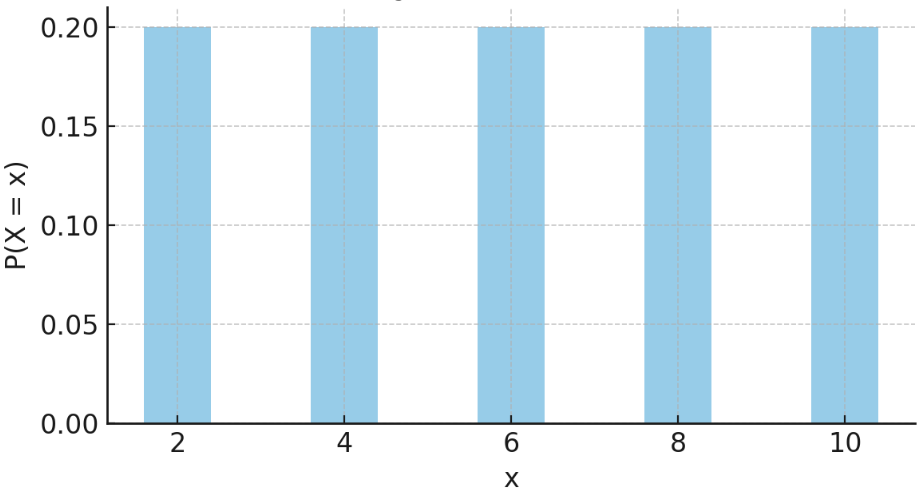
\includegraphics[width=0.75\textwidth]{figuras/dist_disc_uniforme.png}
    \caption{Distribuição Uniforme discreta.}
    \label{fig:dist_disc_uniforme}
\end{figure}

\subsection{Distribuição de Bernoulli}
Dizemos que a variável aleatória $X$ segue o modelo de Bernoulli se atribuímos $0$ à ocorrência de um fracasso ou $1$ à ocorrência de um sucesso, com $p$ representando a probabilidade de sucesso,  
$0 \leq p \leq 1$, e $1 - p$ a probabilidade de fracasso.

A distribuição de probabilidade é dada por:
    $$
    P(X = k) = p^k (1 - p)^{1 - k}, \quad k = 0, 1
    $$

    \begin{center}
    \begin{tabular}{c|cc}
    $X$ & 0 & 1 \\
    \hline
    $P(X = k)$ & $1 - p$ & $p$
    \end{tabular}
    \end{center}

Então,
    $$
    \mathbb{E}[X] = p,
    $$
    $$
    V(X) = p \cdot (1-p)
    $$

A Figura~\ref{fig:dist_disc_bernoulli} apresenta um exemplo de Distribuição de Bernoulli.

\begin{figure}[H]
    \centering
    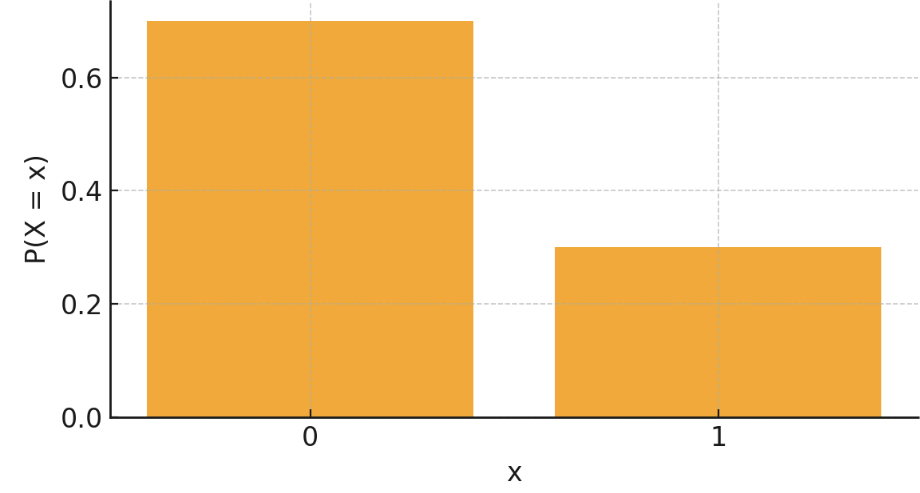
\includegraphics[width=0.75\textwidth]{figuras/dist_disc_bernoulli.png}
    \caption{Distribuição de Bernoulli.}
    \label{fig:dist_disc_bernoulli}
\end{figure}

\subsection{Distribuição Binomial}
O processo estocástico de Bernoulli possui as seguintes propriedades:
\begin{itemize}
    \item O experimento consiste de $n$ tentativas repetidas;
    \item Cada tentativa gera um resultado que pode ser classificado como sucesso ou falha;
    \item A probabilidade de sucesso $p$ se mantém constante de tentativa para tentativa;
    \item As tentativas são feitas de forma independente uma da outra.
\end{itemize}

Seja $X$ uma variável aleatória baseada em $n$ repetições de um processo de Bernoulli.  
Então a probabilidade de obtermos $k$ sucessos em $n$ repetições é dada por:
    $$
    P(X = k) = \binom{n}{k} p^k (1 - p)^{n - k}, \quad k = 0, 1, 2, \ldots, n
    $$,
onde:
    $$
    C_n^k = \binom{n}{k} = \frac{n!}{(n - k)! \, k!}
    $$
é uma combinação de $n$ elementos tomados de $k$ em $k$.

Então,
    $$
    \mathbb{E}[X] = n \cdot p,
    $$
    $$
    V(X) = n \cdot p \cdot (1-p)
    $$

A Figura~\ref{fig:dist_disc_binomial} apresenta um exemplo de Distribuição Binomial.

\begin{figure}[H]
    \centering
    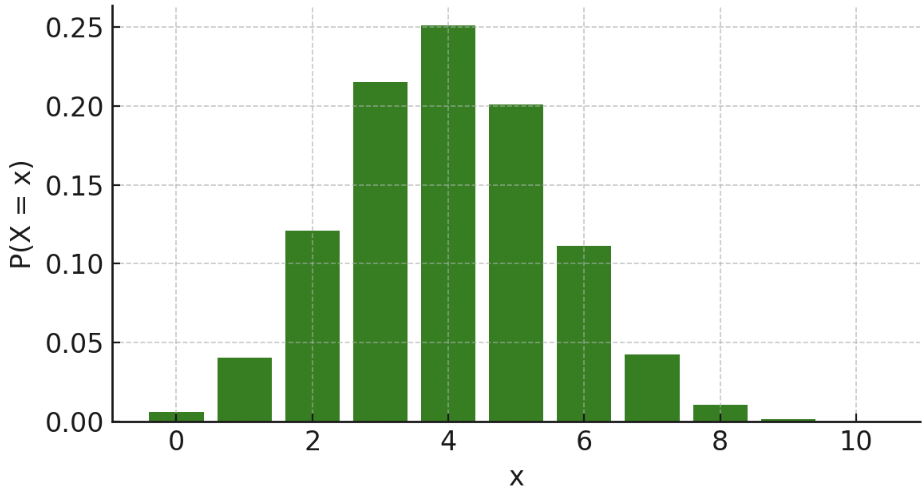
\includegraphics[width=0.75\textwidth]{figuras/dist_disc_binomial.png}
    \caption{Distribuição Binomial.}
    \label{fig:dist_disc_binomial}
\end{figure}

A seguir, apresentamos um exemplo de problema que pode ser modelado por meio da Distribuição Binomial:
\begin{quote}
``Uma urna tem 20 bolas pretas e 30 brancas. Retiram-se 25 bolas com reposição. Qual a probabilidade de que 2 sejam pretas?''
\end{quote}

\subsection{Distribuição de Poisson}
O processo estocástico de Poisson possui as seguintes propriedades:
\begin{itemize}
    \item O processo modela a ocorrência de eventos ao longo do tempo ou espaço contínuo;
    \item Existe uma taxa média constante $\lambda > 0$, que representa o número esperado de eventos por unidade de tempo (ou espaço);
    \item Os eventos ocorrem de forma independente em intervalos disjuntos;
    \item A probabilidade acumulada de ocorrência de eventos aumenta com o tempo.
\end{itemize}

Uma variável aleatória discreta $X$ segue o modelo de Poisson com taxa $\lambda > 0$ se:
    $$
    P(X = k) = \frac{e^{-\lambda} \lambda^k}{k!}, \quad k = 0, 1, 2, \ldots
    $$

Então,
    $$
    \mathbb{E}[X] = \lambda,
    $$
    $$
    V(X) = \lambda
    $$

A Figura~\ref{fig:dist_disc_poisson} apresenta um exemplo de Distribuição de Poisson.

\begin{figure}[H]
    \centering
    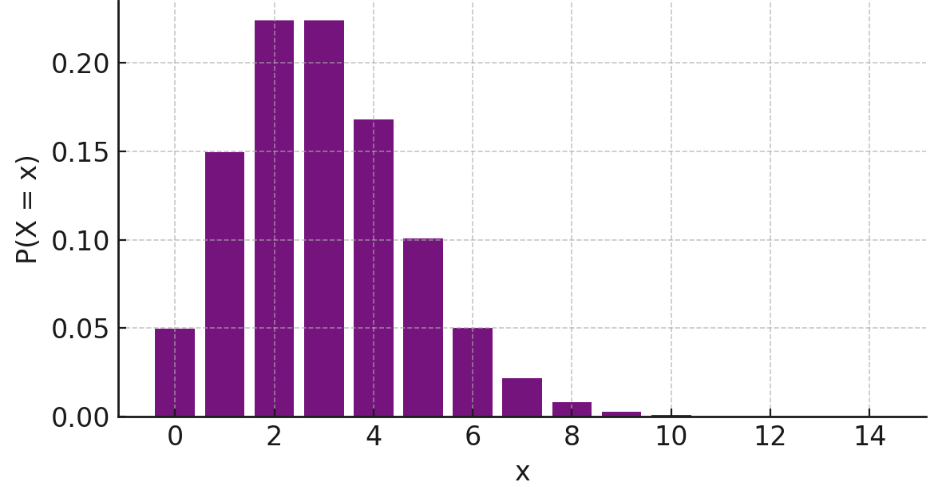
\includegraphics[width=0.75\textwidth]{figuras/dist_disc_poisson.png}
    \caption{Distribuição de Poisson.}
    \label{fig:dist_disc_poisson}
\end{figure}

A seguir, apresentamos um exemplo de problema que pode ser modelado por meio da Distribuição de Poisson:
\begin{quote}
``Numa estrada há 2 acidentes para cada 100 km. Qual a probabilidade de que em 250 km ocorram pelo menos 3 acidentes?''
\end{quote}

\subsection{Lei dos Eventos Raros}
Seja $X$ uma variável aleatória com Distribuição Binomial e $p$ a probabilidade de sucesso. Então,
    $$
    \lim_{n \to \infty} \binom{n}{k} p^k (1 - p)^{n - k} = \frac{e^{-\lambda} \lambda^k}{k!}, \quad k = 0, 1, 2, \ldots,
    $$
onde $\lambda = np$ é constante.

\subsection{Distribuição Geométrica}
A Distribuição Geométrica modela o número de tentativas necessárias até a ocorrência do primeiro sucesso em uma sequência de experimentos de Bernoulli independentes. Suas principais características são:

\begin{itemize}
    \item Cada tentativa resulta em um sucesso (com probabilidade $p$) ou uma falha (com probabilidade $1 - p$);
    \item As tentativas são independentes entre si;
    \item A variável aleatória $X$ representa o número de tentativas até o primeiro sucesso (inclusive o sucesso), ou, equivalentemente, o número de falhas antes do primeiro sucesso.
\end{itemize}

Dizemos que a variável aleatória discreta $X$ segue uma Distribuição Geométrica se:
    $$
    P(X = k) = p(1 - p)^{k - 1}, \quad k = 1, 2, \ldots
    $$

Então,
    $$
    \mathbb{E}[X] = \frac{1}{p},
    $$
    $$
    V(X) = \frac{1 - p}{p^2}
    $$

A Figura~\ref{fig:dist_disc_geometrica} apresenta um exemplo de Distribuição Geométrica.

\begin{figure}[H]
    \centering
    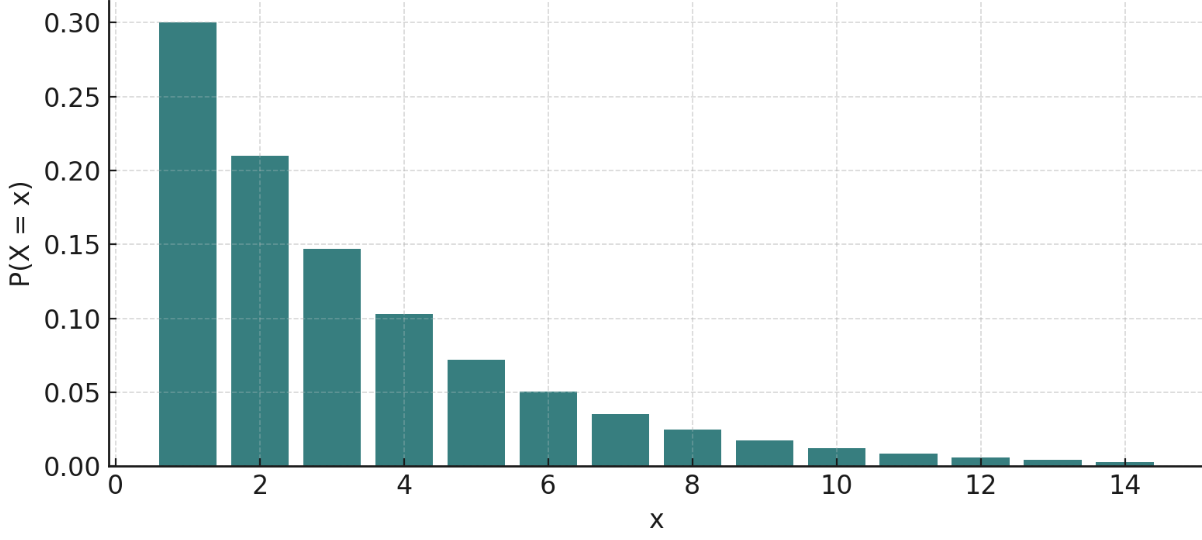
\includegraphics[width=0.75\textwidth]{figuras/dist_disc_geometrica.png}
    \caption{Distribuição Geométrica.}
    \label{fig:dist_disc_geometrica}
\end{figure}

A seguir, apresentamos um exemplo de problema que pode ser modelado por meio da Distribuição Geométrica:
\begin{quote}
``Suponha que temos uma urna com 36 bolas, sendo 27 bolas brancas e 9 pretas. Bolas são retiradas até que uma bola preta apareça. Qual é a probabilidade de que precisaremos de mais de 6 retiradas para sortear a primeira bola preta?''
\end{quote}

\subsection{Distribuição Binomial Negativa}
A Distribuição Binomial Negativa é apropriada para modelar situações em que se deseja saber a probabilidade de que um número fixo de sucessos ocorra na $k$-ésima tentativa, ou seja, quantas falhas ocorrem antes de alcançar um número pré-determinado de sucessos.
\begin{itemize}
    \item Os experimentos são independentes e possuem apenas dois resultados possíveis: sucesso ou falha;
    \item A probabilidade de sucesso $p$ é constante em cada tentativa;
    \item O processo continua até que um número fixo de sucessos seja alcançado.
\end{itemize}

Seja $X$ o número de repetições necessárias a fim de que ocorram exatamente $r$ sucessos, de modo que o $r$-ésimo sucesso ocorra na $k$-ésima tentativa. Então,
    $$
    P(X = k) = \binom{k - 1}{r - 1} p^r (1 - p)^{k - r}, \quad k = r, r + 1, \ldots
    $$

A Figura~\ref{fig:dist_disc_binomial_negativa} apresenta um exemplo de Distribuição Binomial Negativa.

\begin{figure}[H]
    \centering
    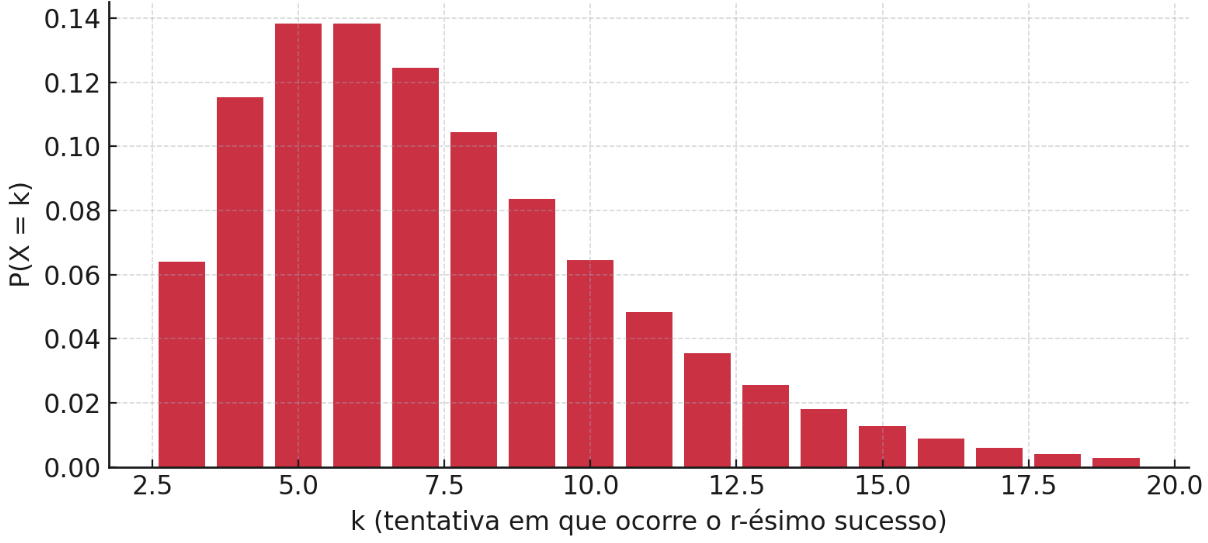
\includegraphics[width=0.75\textwidth]{figuras/dist_disc_binomial_negativa.png}
    \caption{Distribuição Binomial Negativa.}
    \label{fig:dist_disc_binomial_negativa}
\end{figure}

A seguir, apresentamos um exemplo de problema que pode ser modelado por meio da Distribuição Binomial Negativa:
\begin{quote}
``Em uma série da liga de futebol amador de uma cidade, o time que ganhar quatro jogos em sete será o vencedor. Suponha que o time
A tenha probabilidade $p = 0,6$ de ganhar do time B. Qual é a probabilidade de que A vença a série em seis jogos?''
\end{quote}

\subsection{Distribuição Hipergeométrica}
A Distribuição Hipergeométrica é semelhante à Distribuição Binomial, porém com uma diferença essencial: as retiradas são feitas sem reposição. Enquanto a Distribuição Binomial assume que cada tentativa é independente e a probabilidade de sucesso permanece constante (devido à reposição), a Distribuição Hipergeométrica modela situações em que a probabilidade de sucesso varia a cada retirada, pois os elementos não são devolvidos ao conjunto.

Considere um conjunto de $N$ objetos, dos quais $N_1$ são do tipo 1 e $N_2 = N - N_1$ são do tipo 2.  
Para um sorteio de $n$ objetos ($n < N$), sem reposição, seja $X$ a variável aleatória que define o número de objetos do tipo 1 sorteados.  
Então, a probabilidade de sortearmos $k$ objetos do tipo 1 é:
    $$
    P(X = k) = \frac{\binom{N_1}{k} \binom{N - N_1}{n - k}}{\binom{N}{n}}, \quad k = 0, 1, \ldots, n
    $$

A Figura~\ref{fig:dist_disc_hipergeometrica} apresenta um exemplo de Distribuição Hipergeométrica.

\begin{figure}[H]
    \centering
    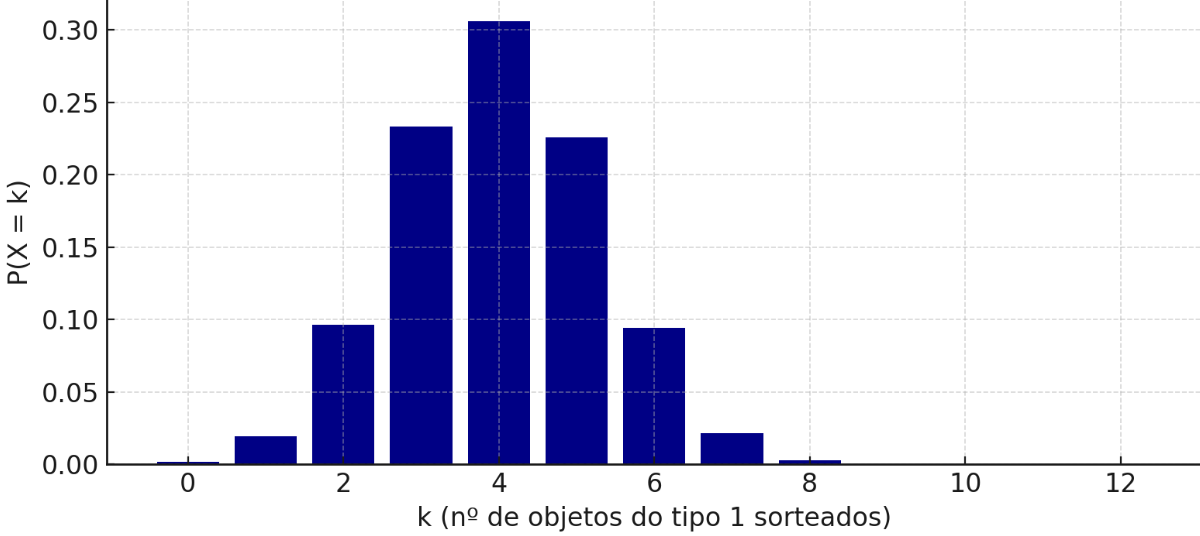
\includegraphics[width=0.75\textwidth]{figuras/dist_disc_hipergeometrica.png}
    \caption{Distribuição Hipergeométrica.}
    \label{fig:dist_disc_hipergeometrica}
\end{figure}

A seguir, apresentamos um exemplo de problema que pode ser modelado por meio da Distribuição Hipergeométrica:
\begin{quote}
``Numa urna há 40 bolas brancas e 60 pretas. Retiram-se 20 bolas. Qual a probabilidade de que ocorram no mínimo 2 bolas brancas, considerando extrações sem reposição?''
\end{quote}

\section{Modelos Probabilísticos Contínuos}

\subsection{Distribuição Uniforme Contínua}
Uma variável aleatória contínua $X$ segue uma Distribuição Uniforme se sua função densidade de probabilidade é dada por:
    $$
    f(x) = \begin{cases}
    \frac{1}{b - a}, & x \in [a, b] \\
    0, & x \notin [a, b]
    \end{cases}
    $$
Então,
    $$
    \mathbb{E}[X] = \frac{a + b}{2},
    $$
    $$
    V(X) = \frac{(b - a)^2}{12}
    $$
A Figura~\ref{fig:dist_cont_uniforme} apresenta um exemplo de Distribuição Uniforme contínua.

\begin{figure}[H]
    \centering
    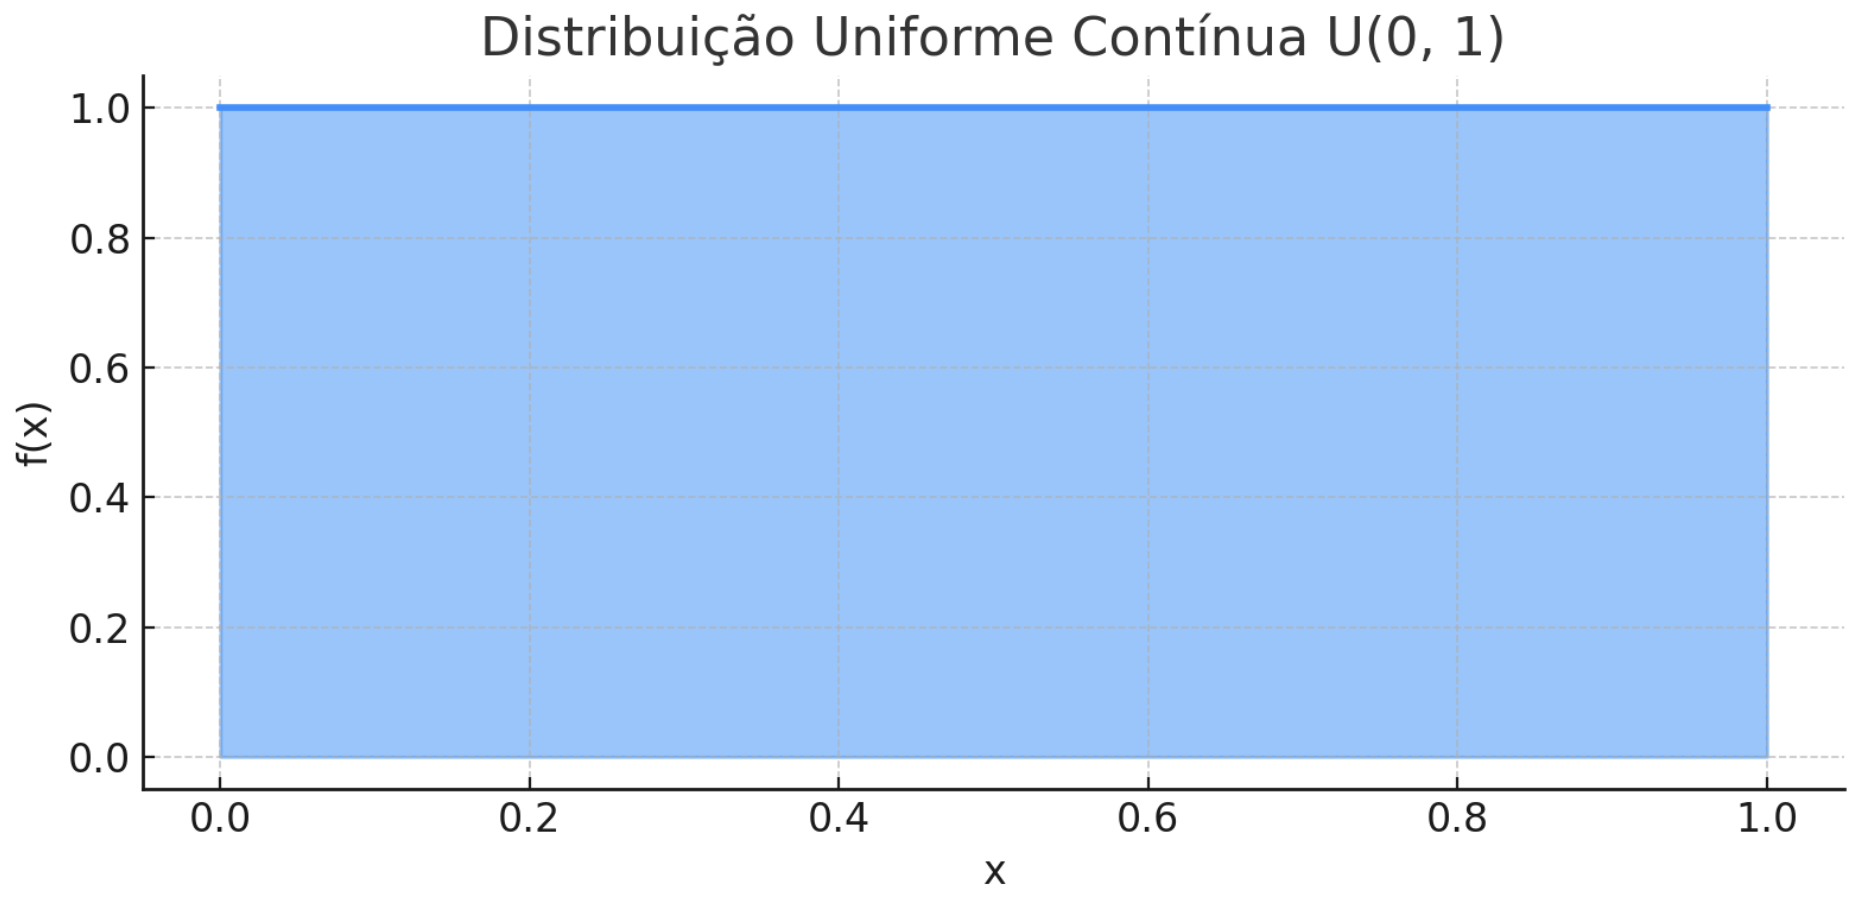
\includegraphics[width=0.75\textwidth]{figuras/dist_cont_uniforme.png}
    \caption{Distribuição Uniforme contínua.}
    \label{fig:dist_cont_uniforme}
\end{figure}

\subsection{Distribuição Normal}
Uma variável aleatória contínua $X$ que tome todos os valores na reta real segue a Distribuição Normal (ou Gaussiana) se sua função densidade de probabilidade é definida por:
    $$
    f(x) = \frac{1}{\sigma \sqrt{2\pi}} \exp\left[ -\frac{1}{2} \left( \frac{x - \mu}{\sigma} \right)^2 \right], \quad -\infty < x < \infty
    $$
onde $\mu = E[X]$ e $\sigma^2 = V(X) > 0$.


A Distribuição Normal apresenta as seguintes propriedades:
\begin{itemize}
    \item $f(x)$ é simétrica em relação à $\mu$.
    \item $f(x) \to 0$ quando $x \to \pm\infty$.
    \item O valor máximo de $f(x)$ ocorre em $x = \mu$.
\end{itemize}


Se $X$ é uma variável aleatória contínua com distribuição normal, $X \sim \mathcal{N}(\mu, \sigma^2)$, e se $Y = aX + b$, com $a$ e $b$ constantes, então
    $$
    Y \sim \mathcal{N}(a\mu + b, a^2\sigma^2).
    $$
Seja $X \sim \mathcal{N}(\mu, \sigma^2)$. Se
    $$
    Z = \frac{X - \mu}{\sigma},
    $$
então $Z \sim \mathcal{N}(0, 1)$.

Assim,
\begin{align*}
    P(a \leq X \leq b) &= P\left( \frac{a - \mu}{\sigma} \leq \frac{X - \mu}{\sigma} \leq \frac{b - \mu}{\sigma} \right) \\
    &= P\left( \frac{a - \mu}{\sigma} \leq Z \leq \frac{b - \mu}{\sigma} \right) \\
    &= P(X \leq b) - P(X \leq a).
\end{align*}

A tabela Normal pode ser acessada através do link \url{https://en.wikipedia.org/wiki/Standard_normal_table#Table_examples}.

A Figura~\ref{fig:dist_cont_normal} apresenta um exemplo de Distribuição Normal.

\begin{figure}[H]
    \centering    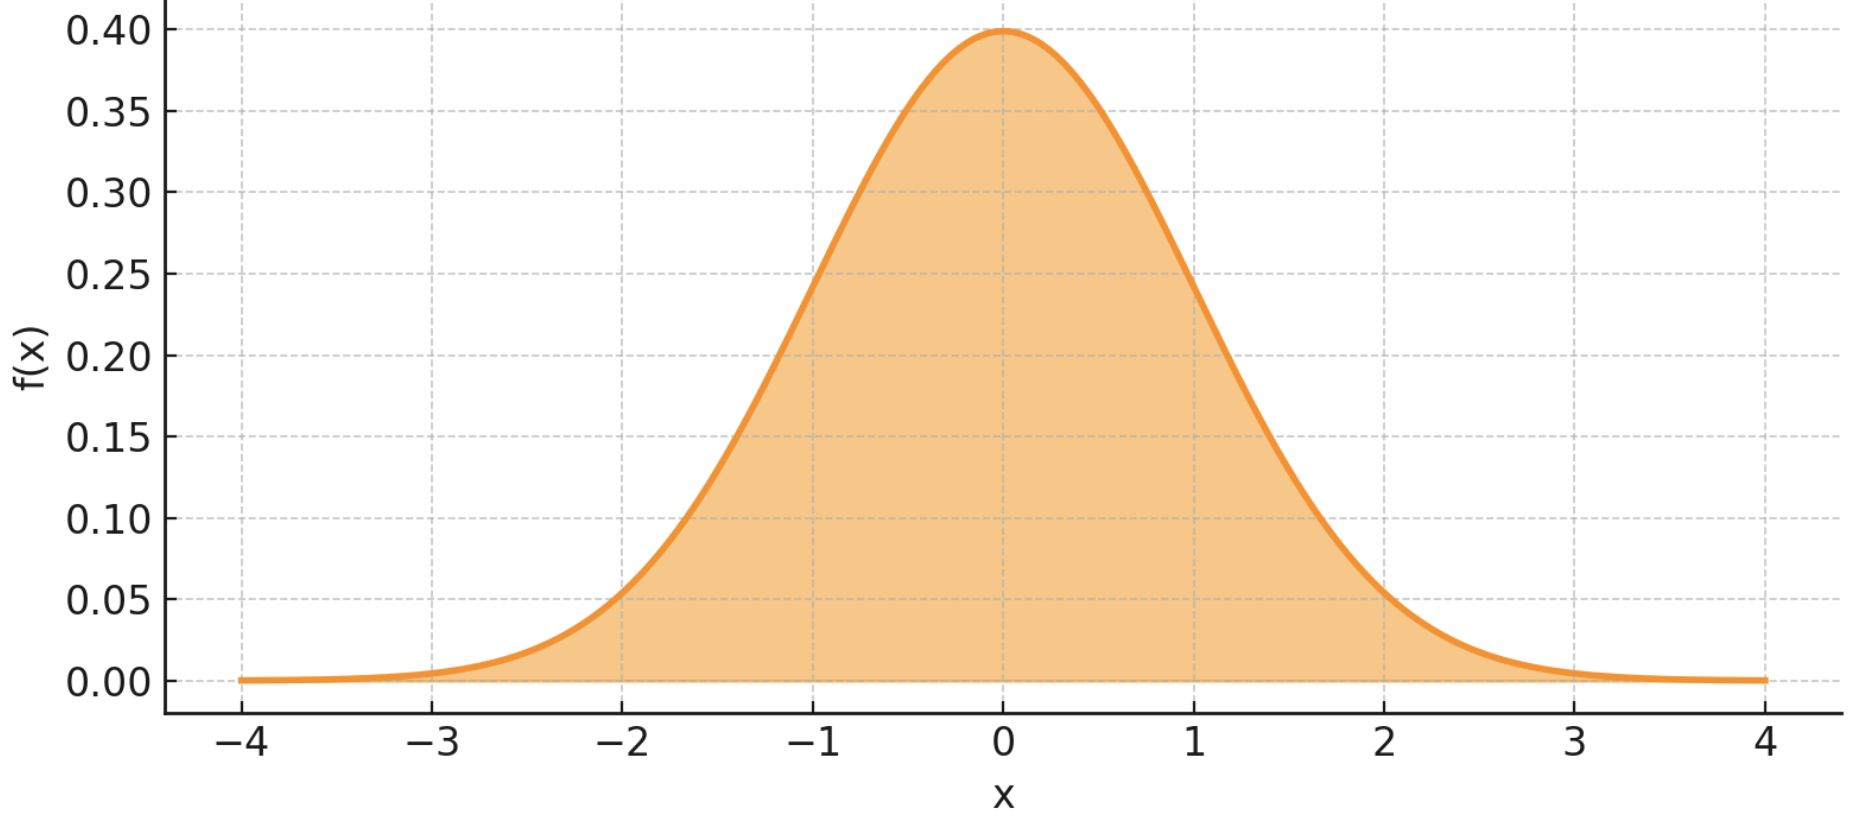
\includegraphics[width=0.75\textwidth]{figuras/dist_cont_normal.png}
    \caption{Distribuição Normal.}
    \label{fig:dist_cont_normal}
\end{figure}

\subsection{Distribuição Exponencial}
Uma variável aleatória contínua $X$ segue o modelo exponencial se sua função densidade de probabilidade é dada por:
    $$
    f(x) = 
    \begin{cases}
    \lambda e^{-\lambda x}, & x \geq 0 \\
    0, & x < 0
    \end{cases}
    $$
onde $\lambda > 0$ e $-\infty < x < \infty$.

Então,
    $$
    E[X] = \frac{1}{\lambda},
    $$
    $$
    V(X) = \frac{1}{\lambda^2}
    $$

A Distribuição Exponencial apresenta a propriedade de ``ausência de memória'', isto é:
    $$
    P(X \geq t + s \mid X \geq s) = P(X \geq t)
    $$

A Figura~\ref{fig:dist_cont_exponencial} apresenta um exemplo de Distribuição Exponencial.

\begin{figure}[H]
    \centering    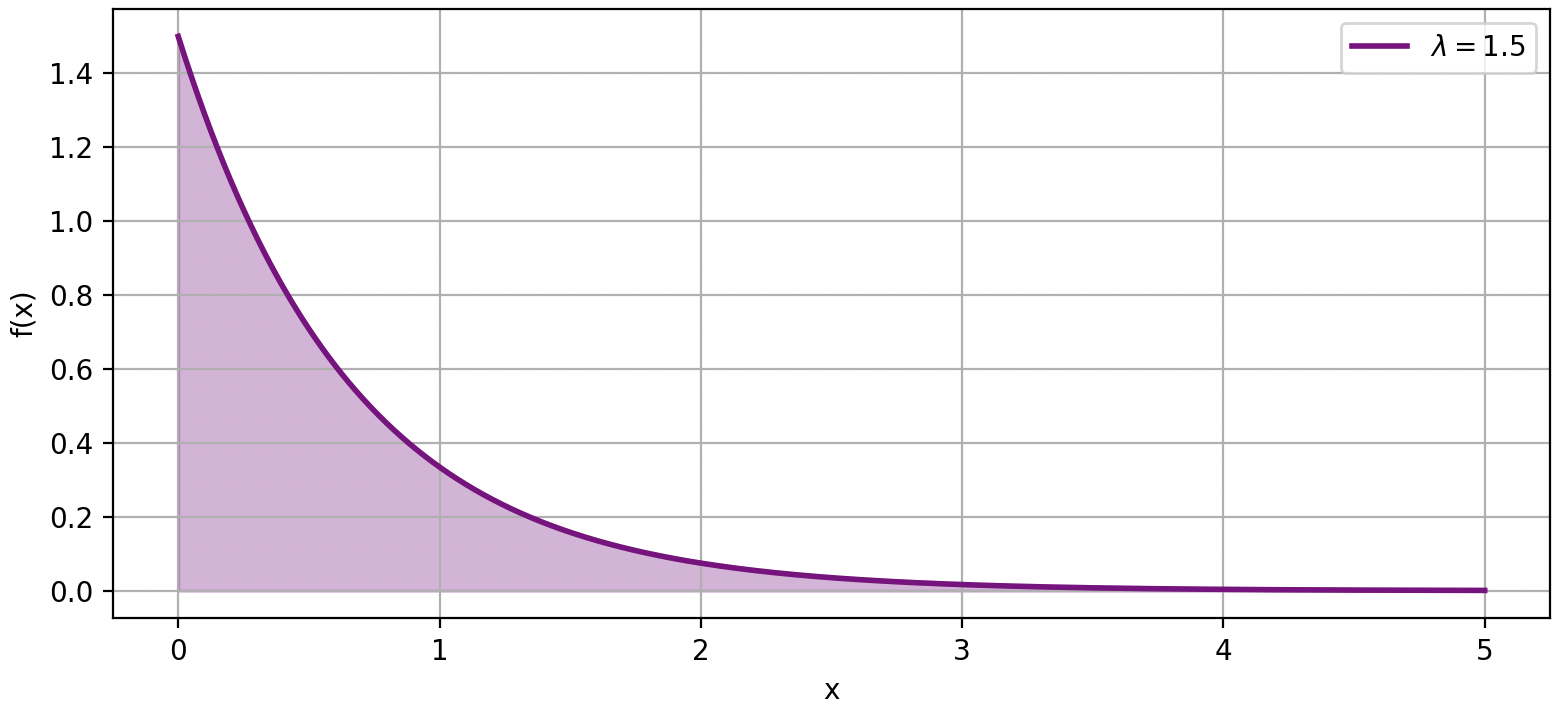
\includegraphics[width=0.75\textwidth]{figuras/dist_cont_exponencial.png}
    \caption{Distribuição Exponencial.}
    \label{fig:dist_cont_exponencial}
\end{figure}

\subsection{Distribuição Gama}
Uma variável aleatória contínua $X$ tem Distribuição Gama com parâmetros $\lambda > 0$ e $\alpha > 0$, se sua função densidade de probabilidade é dada por:
    $$
    f(x) =
    \begin{cases}
    \frac{\lambda^\alpha}{\Gamma(\alpha)} x^{\alpha - 1} e^{-\lambda x}, & x \geq 0, \\
    0, & x < 0,
    \end{cases}
    $$
onde $\Gamma$ é a função gama:
    $$
    \Gamma(\alpha) = \int_0^{\infty} t^{\alpha - 1} e^{-t} \, dt.
    $$

Então,
    $$
    E[X] = \frac{\alpha}{\lambda},
    $$
    $$
    V(X) = \frac{\alpha}{\lambda^2}
    $$

Se $\alpha$ for um número inteiro positivo, a distribuição representará uma distribuição Erlang, ou seja, a soma de $\alpha$ variáveis aleatórias independentes distribuídas exponencialmente, cada uma delas com uma média $\theta = 1/\lambda$.

A Figura~\ref{fig:dist_cont_gama} apresenta um exemplo de Distribuição Gama.

\begin{figure}[H]
    \centering    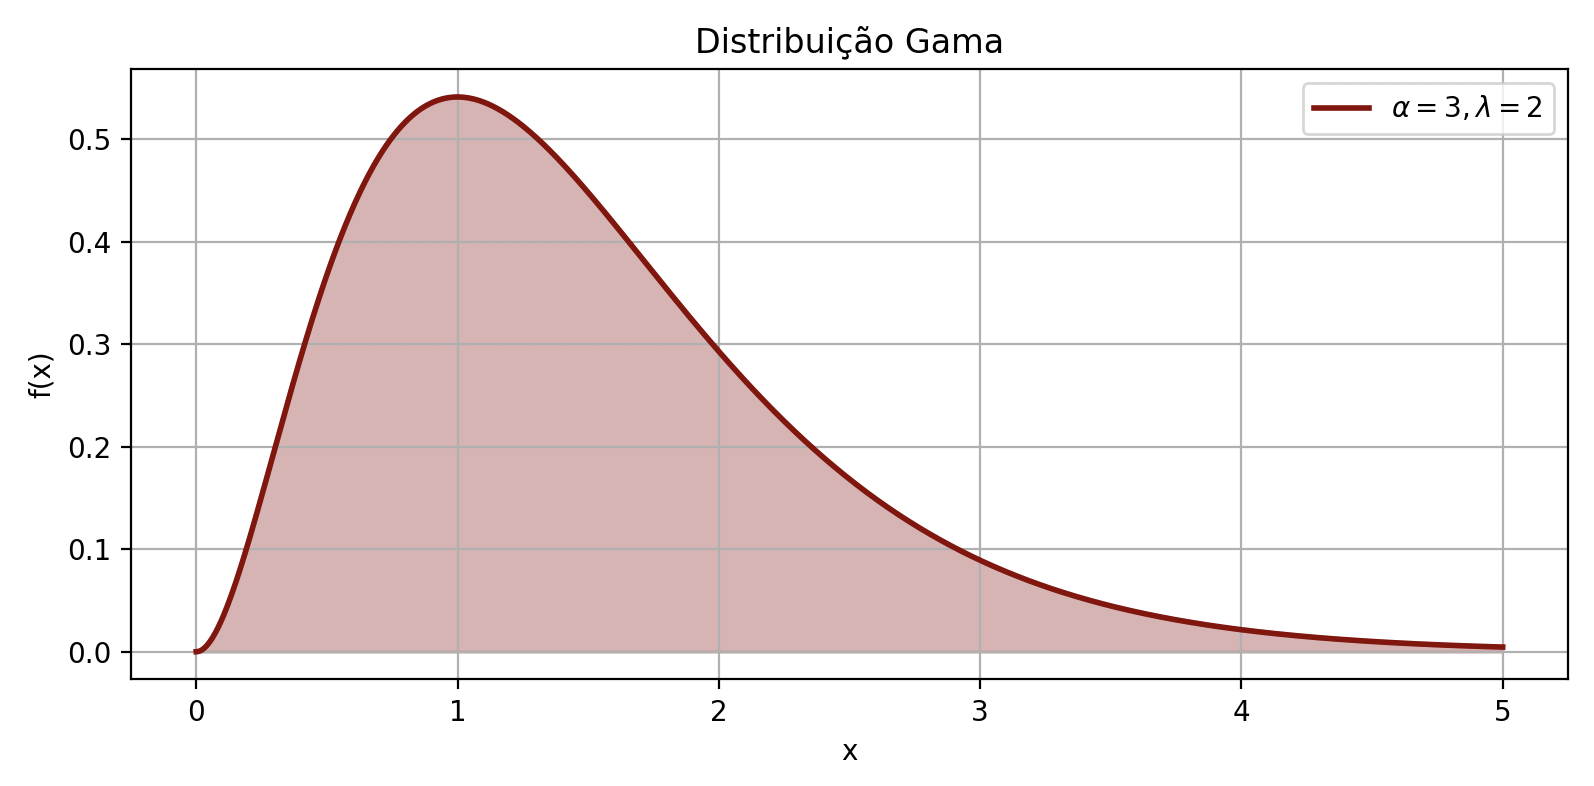
\includegraphics[width=0.75\textwidth]{figuras/dist_cont_gama.png}
    \caption{Distribuição Gama.}
    \label{fig:dist_cont_gama}
\end{figure}

\subsection{Distribuição Qui-Quadrado}
A variável aleatória contínua $X$ segue a Distribuição Qui-Quadrado (denominada $\chi^2$) se sua função densidade de probabilidade é dada por:
    $$
    f(x) = 
    \begin{cases}
    \frac{x^{k/2 - 1} e^{-x/2}}{2^{k/2} \Gamma(k/2)}, & x > 0, \\
    0, & x \leq 0,
    \end{cases}
    $$

A Distribuição Qui-Quadrado é definida pela soma de $k$ distribuições normais padronizadas e independentes. Ou seja, $X$ tem Distribuição Qui-Quadrado com $k$ graus de liberdade se
    $$
    X = \sum_{i=1}^{k} Z_i^2,
    $$
onde $Z_1, Z_2, \ldots, Z_k$ são variáveis aleatórias com distribuição normal padronizada,
    $$
    Z_i \sim \mathcal{N}(\mu = 0, \sigma^2 = 1), \quad i = 1, \ldots, k.
    $$

Para denominar que $X$ segue uma Distribuição Qui-Quadrado, usamos $X \sim \chi^2(k)$ ou $X \sim \chi_k^2$.

A Figura~\ref{fig:dist_cont_quiquadrado} apresenta um exemplo de Distribuição Qui-Quadrado.

\begin{figure}[H]
    \centering    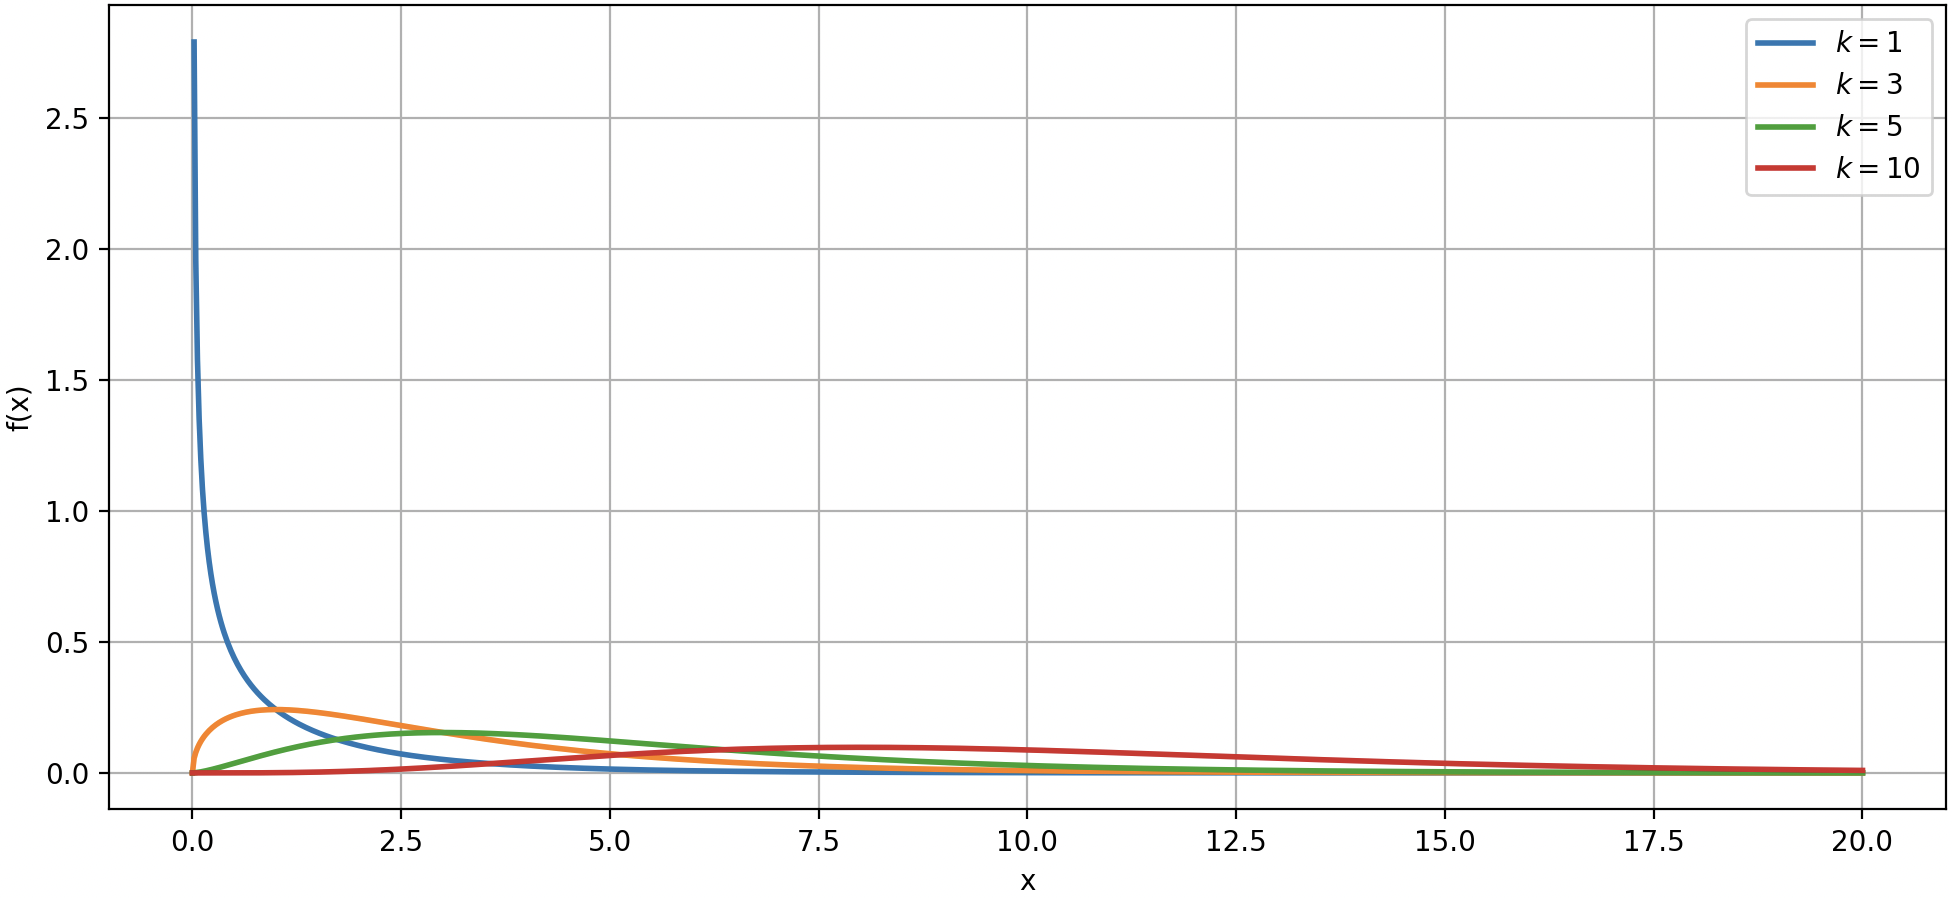
\includegraphics[width=0.75\textwidth]{figuras/dist_cont_quiquadrado.png}
    \caption{Distribuição Qui-Quadrado.}
    \label{fig:dist_cont_quiquadrado}
\end{figure}

\subsection{Distribuição Beta}
Seja $X$ uma variável aleatória contínua limitada em $[0,1]$. Dizemos que $X$ segue uma Distribuição Beta se sua função densidade de probabilidade é dada por:
    $$
    f(x) =
    \begin{cases}
    \frac{1}{B(\alpha, \beta)} x^{\alpha - 1} (1 - x)^{\beta - 1}, & 0 < x < 1, \\
    0, & \text{caso contrário},
    \end{cases}
    $$
onde $\alpha, \beta > 0$ e
    $$
    B(\alpha, \beta) = \int_0^1 x^{\alpha - 1} (1 - u)^{\beta - 1} \, du,
    $$
é a função beta, que atua como uma constante de normalização para que a área da função densidade de probabilidade seja igual a um.

A Figura~\ref{fig:dist_cont_beta} apresenta um exemplo de Distribuição Beta.

\begin{figure}[H]
    \centering    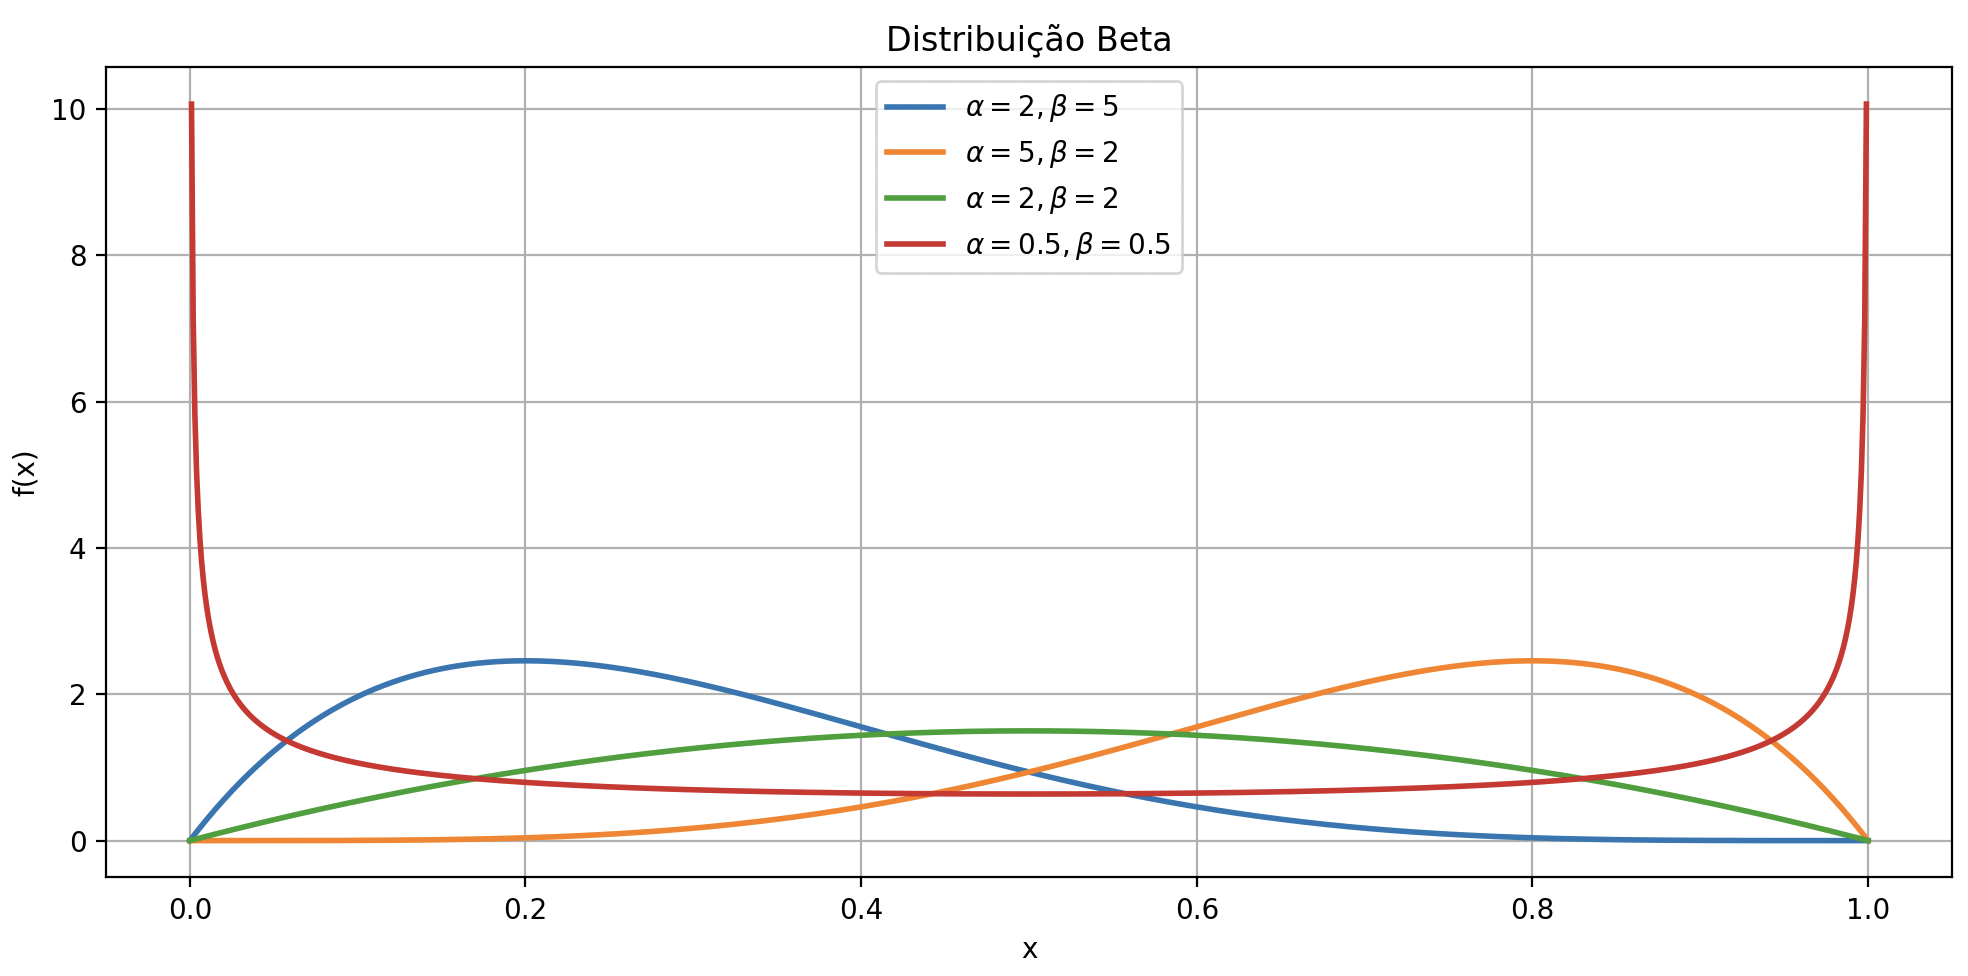
\includegraphics[width=0.75\textwidth]{figuras/dist_cont_beta.png}
    \caption{Distribuição Beta.}
    \label{fig:dist_cont_beta}
\end{figure}

\subsection{Distribuição t de Student}
A variável aleatória $X$ tem Distribuição t de Student com $\nu$ graus de liberdade se sua função densidade de probabilidade é dada por:
    $$
    f(x) = \frac{\Gamma\left(\frac{\nu+1}{2}\right)}{\sqrt{\nu \pi} \, \Gamma\left(\frac{\nu}{2}\right)} \left(1 + \frac{x^2}{\nu} \right)^{-\frac{\nu+1}{2}}, \quad -\infty < x < \infty
    $$
onde $\Gamma$ é a função gama:
    $$
    \Gamma(\alpha) = \int_0^{\infty} t^{\alpha - 1} e^{-t} \, dt
    $$

Quando aumentamos $\nu$, a distribuição se aproxima da Distribuição Normal.

A Figura~\ref{fig:dist_cont_tstudent} apresenta um exemplo de Distribuição t de Student.

\begin{figure}[H]
    \centering    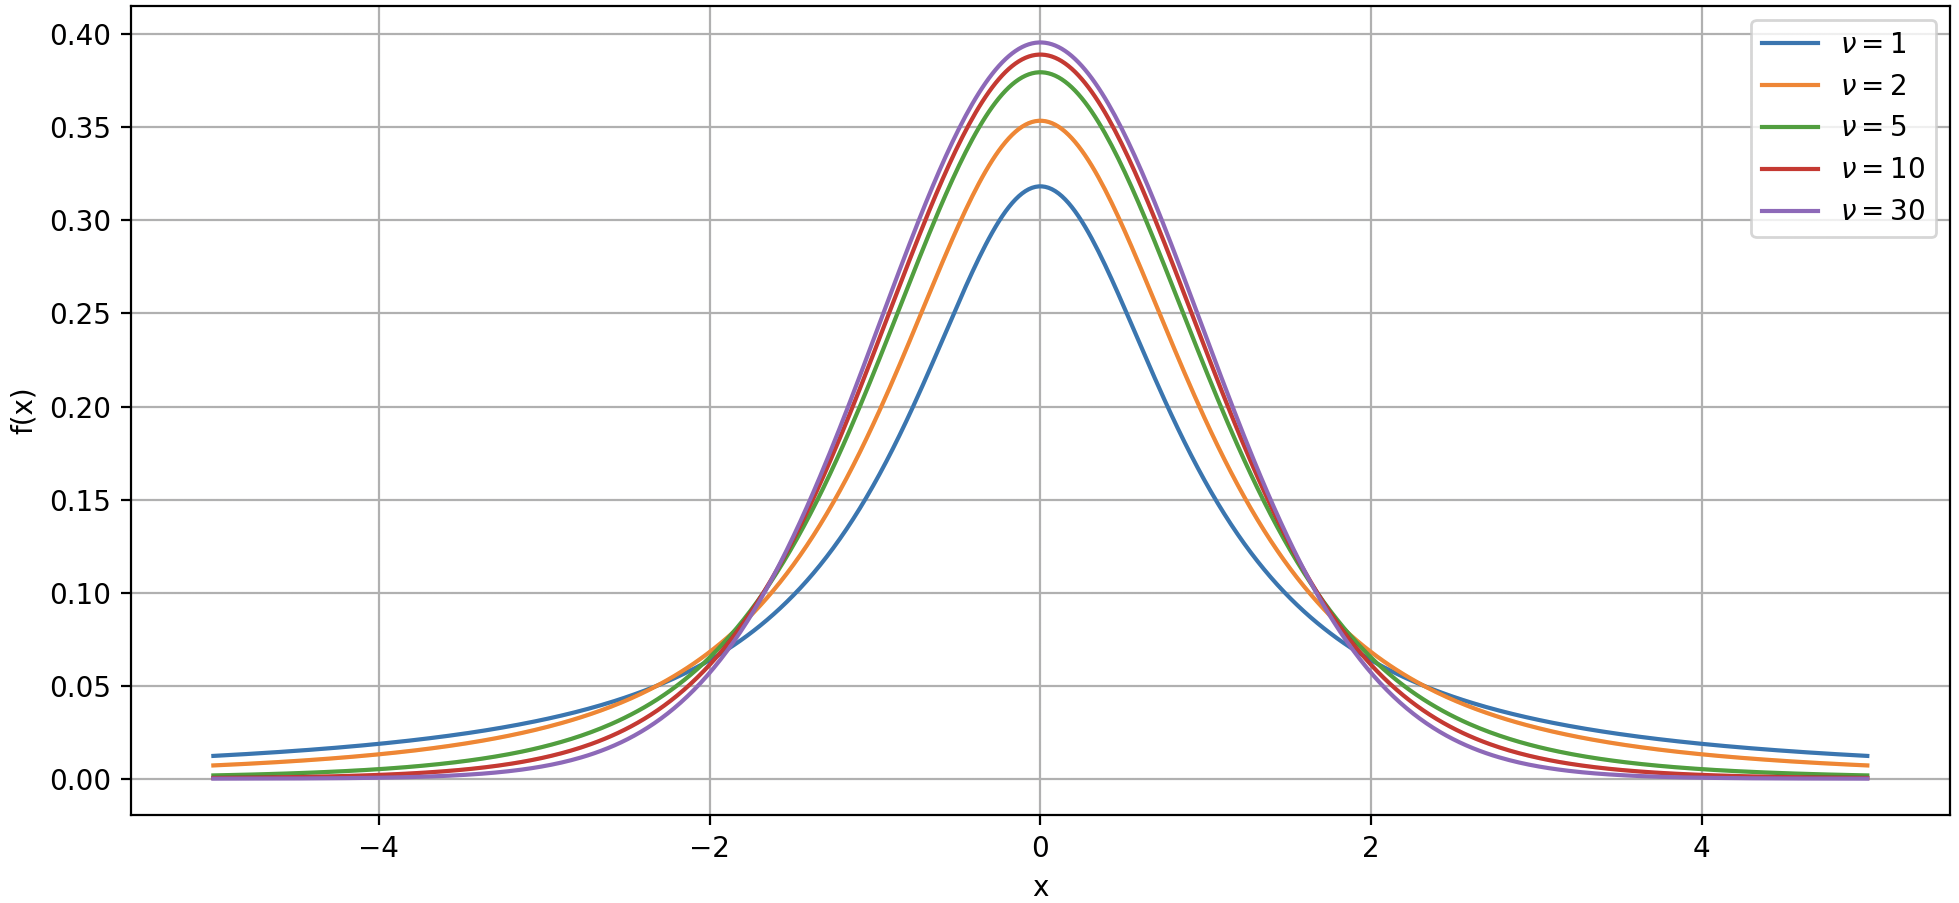
\includegraphics[width=0.75\textwidth]{figuras/dist_cont_tstudent.png}
    \caption{Distribuição t de Student.}
    \label{fig:dist_cont_tstudent}
\end{figure}

\end{document}
